\begin{figure}
    \centering
    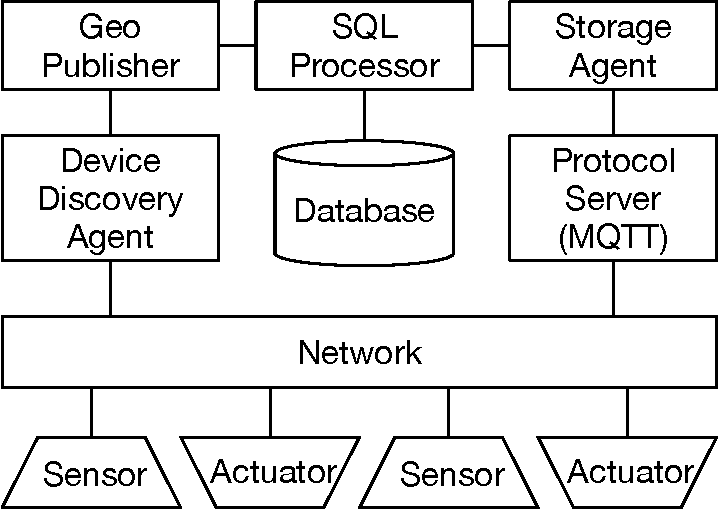
\includegraphics[width=0.8\linewidth]{figs/acps.pdf}%
    \caption{The conceptual diagram of an autonomous cyber-physical system (ACPS).}\label{fig:acps}%
\end{figure}

\begin{figure}
    \centering
    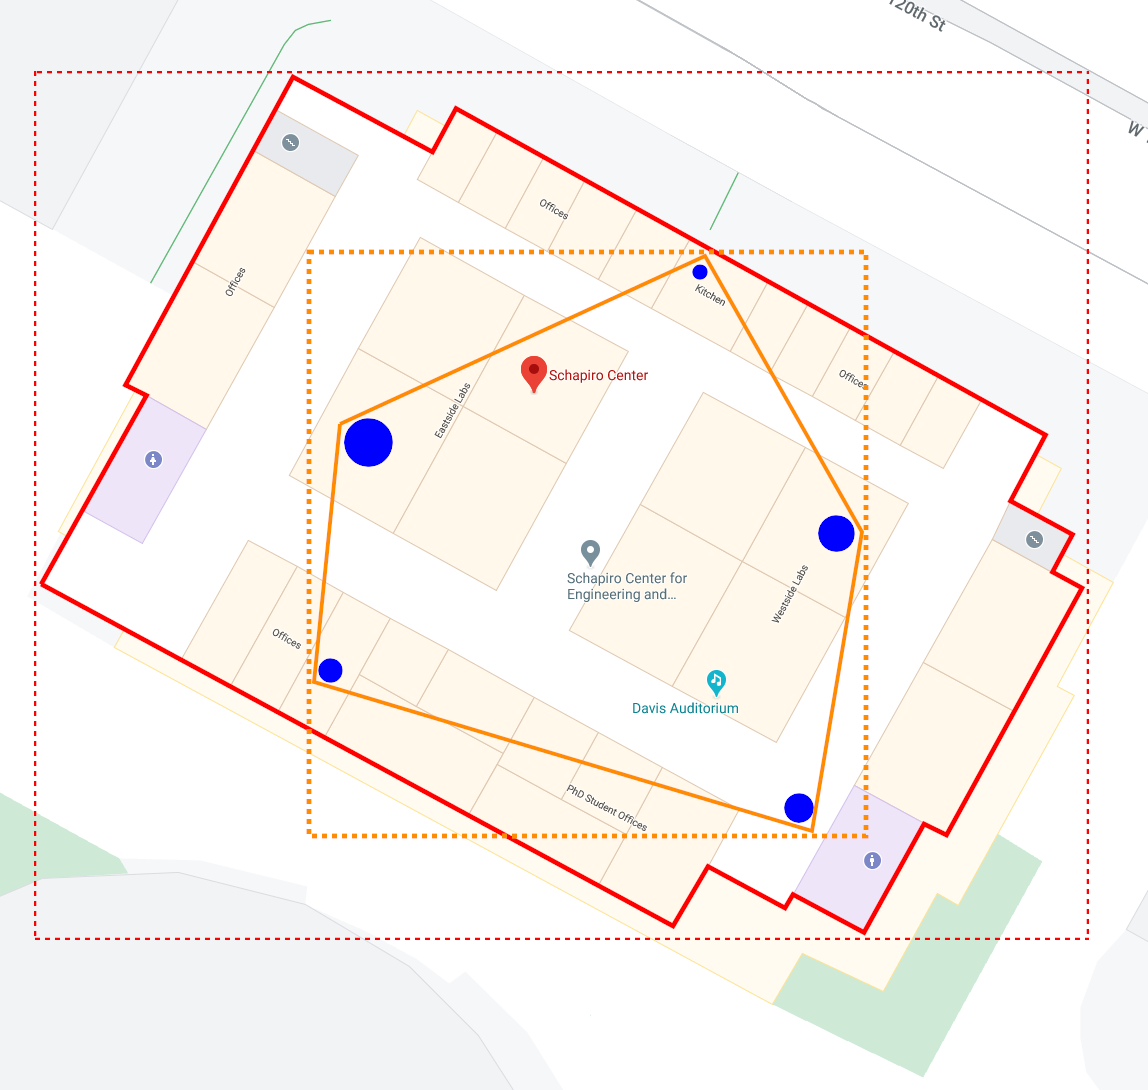
\includegraphics[width=1\linewidth]{figs/acps-coverage.png}%
    \caption{Device location estimates (blue), computed coverage region (orange), manually configured coverage region (red). Corresponding bounding boxes are shown with dotted lines.}\label{fig:acps-coverage}%
\end{figure}


An \gls{acps} is a collection of networked sensors, actuators, and related infrastructure managed by a common administrative entity. \cref{fig:acps} shows the conceptual internal architecture of the \gls{acps}. The sensors in a smart home would typically belong one \gls{acps}. The infrastructure on a large university campus may be divided among several \glspl{acps}, e.g., by building or department. Event in small deployments it may be advantageous to operate multiple related \glspl{acps} to limit the scope of potential failures or to split the infrastructure into public and private.

Each device within the \gls{acps} is associated with a \emph{storage node}. The node provides persistent storage and a query interface for the data (measurements) generated by associated devices. The association is administrative and can change over time. While it might be best to place the storage node close to the sensors, e.g., in the same \gls{lan}, it is not required. The storage node could also be provided in the form of a cloud-based service communicating with its associated sensors over a \gls{wan}. The former approach can be realized by placing the storage on an \gls{iot} gateway. The latter accommodates sensors that maintain a persistent connection to manufacturer-operated cloud infrastructure.

The \gls{acps} includes various sensor protocol servers (\emph{MQTT Server} in \cref{fig:acps}), a local \gls{sql} database, and a \emph{storage agent} process. The agent obtains measurement data from sensors and writes the data into the database. The exact mechanism is out of scope and will depend on the facilities provided by sensor protocol (push or pull), the configuration of the \gls{acps}, and local administrator policies (e.g., measurement intervals).

% Some background on uncertainty/radius https://en.wikipedia.org/wiki/Geo_URI_scheme

We assume the \gls{acps} can estimate the \gls{wgs} 84\footnote{We choose \gls{wgs} 84 because that is the coordinate system used by the \gls{gps} and it is widely supported. Other coordinate systems exist. Alternatively, one could also use a planar (Euclidean) coordinate system which would simplify some of the math in \gls{sql} spatial.} coordinates of each associated device. It maintains a \emph{location estimate} for each device in the form of a $(latitude, longitude, uncertainty)$ triplet represented with a geo \gls{uri}~\cite{rfc5870}. The uncertainty component is expressed at a confidence of 95\% or higher. Geometrically, the location estimate can be represented by a disk with the radius $uncertainty$. A location estimate with large uncertainty (coarse location) as provided by, e.g., Wi-Fi or \gls{ip} address positioning services, is sufficient for many applications. The means through which location estimates are obtained is out of the scope of this paper. In \cref{fig:acps-coverage}, the location estimates are shown in blue.

% TODO: how is the published service descriptor authenticated?

The \emph{coverage region} of an \gls{acps} is a geographic region that fully contains the location estimates of all the devices associated with the \gls{acps}. The coverage region is not necessarily the smallest such region and could be defined administratively, e.g., based on a building floor plan. If not provided, the \gls{acps} computes its coverage region as a convex envelope over the location estimates of all of its devices. The coverage region may change over time as device come, go, or move. The coverage regions of multiple \glspl{acps} may overlap.

The \emph{bounding box} of an \gls{acps} is the minimum rectangle that fully contains the \glsfirst{acps}['s] coverage region. Both the coverage region and the bounding box are represented with a single GeoJSON~\cite{rfc7946} object. The "bbox" property must be present and represents the \gls{acps}['s] bounding box.

The \emph{service descriptor} of an \gls{acps} is a digitally signed \gls{json}~\cite{rfc8259} object that binds the \gls{acps}['s] coverage region with additional information describing the \gls{acps} such as its contact \gls{uri}, available sensor or actuator types, or a human-friendly name:
\begin{minted}[fontsize=\footnotesize]{JSON}
{ "@type": "ServiceDescriptor",
  "@context": "https://schema.org/SynSQL",
  "displayName": "IRT Lab Sensors",
  "lastUpdated": "<ISO timestamp>",
  "expires": "<ISO timestamp>",
  "coverageRegion": {
      "type": "Polygon",
      "bbox": [-10.0, -10.0, 10.0, 10.0],
      "coordinates": [] },
  "private": false,
  "contact": "wss://as-123.example.com:8443",
  "sensorTypes": [
      "urn:sensor:environmental:indoor",
      "urn:sensor:security",
      "urn:sensor:occupancy" ],
  "signature": {} }
\end{minted}

The \gls{acps} publishes (\emph{GeoPublisher} in \cref{fig:acps}) its service descriptor in the \gls{gd} discussed later.  The service descriptor should provide sufficient information for the clients to submit \gls{sql} queries to the \gls{acps}. We expect the service descriptors to be updated infrequently. The record provides attributes that enable caching.

The \gls{acps} provides a public \gls{sql}[-based] interface (\emph{SQL Processor} in \cref{fig:acps}) to the stored sensor and actuator data. An advantage of \gls{sql}[-based] interface, as opposed to just publishing the underlaying data, is that: 1) query computation can be moved to data, 2) dynamic access control policies can be applied, 3) information hiding can be enforced by the \gls{acps}. For simplicity, we assume that all \glspl{acps} use a common data model (discussed elsewhere in the paper).

At a minimum, the \gls{acps} must support basic standards-based \gls{sql}. The \gls{acps} can also indicate support for the spatial \gls{sql} extension in the published service descriptor. In that case, the \gls{acps} may receive \gls{sql} queries with spatial predicates\footnote{The idea here is that the \gls{acps} can indicate whether its storage node is willing to process spatial \gls{sql} queries. If it is, it may receive full \gls{sql} queries from query coordinators and will be expected to evaluate spatial predicates using supplied geospatial data. That allows moving the computationally expensive spatial operations from the coordinator to storage nodes, i.e., close to the data.}. This is useful, for example, if the \gls{acps}['s] storage node has private spatial objects, e.g., derived from a building floor plan. This feature allows the clients to query sensor measurements with respect to such data, without necessarily being able to obtain the spatial objects for privacy reasons.
